\documentclass{article}
\usepackage{fullpage,graphicx}
\usepackage{amsmath,amsfonts,amsthm,amssymb,multirow}
\usepackage{algorithmic}
\usepackage{tikz}
\usepackage[ruled,vlined,commentsnumbered,titlenotnumbered]{algorithm2e}
\newcommand{\expecting}[1]{\noindent\textbf{[We are expecting: #1]}}
\newcommand{\hint}[1]{\noindent\textbf{[HINT: #1]}}
\newcommand{\pts}[1]{\textbf{(#1 pt.)}}

\begin{document}
\noindent
CS 161 \hfill \textbf{Problem Set 2} \newline 
{Autumn 2017} \hfill \textbf{Due:} Friday October 13, 2017, at 3pm on Gradescope

\noindent
\rule{\linewidth}{0.4pt}

\section*{Exercises}
Exercises should be completed \textbf{on your own.}  

\noindent
\rule{\linewidth}{0.4pt}
\begin{enumerate}
\item\pts{2} In your pre-lecture Exercise for Lecture 3, you saw two different proofs that the solution to the recurrence relation $T(n) = 2\cdot T(n/2) + n$ with $T(1) = 1$, was exactly $T(n) = n(1 + \log(n))$, when $n$ was a power of two.
\begin{enumerate}
	\item What is the exact solution to $T(n) = 2 \cdot T(n/2) + n$ with $T(1) = 2$, when $n$ is a power of $2$?
	\item What is the exact solution to $T(n) = 2\cdot T(n/2) + 2n$ with $T(1) = 1$, when $n$ is a power of $2$?
\end{enumerate}
\expecting{ Your answer, with a convincing argument (it does not need to be a formal proof).  Notice that we want the exact answer, so don't give a $O()$ statement. }


\item\pts{2} Consider the recurrence relation $T(n) = T(n-1) + n$ with $T(1) = 1$.  Your friend claims that $T(n) = O(n)$, and offers the following justification:

\begin{quote}
Let's use the Master Theorem with $a = 1$, $b = \frac{n}{n-1}$, and $d = 1$.  
This applies since \[ \frac{n}{b} = n \cdot \left( \frac{n-1}{n} \right) = n-1. \]
Then we have $a < b^d$, so the Master Theorem says that
$T(n) = O(n^d) = O(n).$
\end{quote}

What's wrong with your friend's argument, and what is the correct answer?

\hint{It is totally fine to apply the Master Theorem when $b$ is a fraction; that's not the problem.}

\expecting{A clear identification of the faulty logic above; your solution to this recurrence (you may use asymptotic notation\footnote{Unless specified otherwise, in every problem set, when we ask for an answer in asymptotic notation, we are asking either for a $\Theta(\cdot)$ result, or else the tightest $O(\cdot)$ result you can come up with.}) and a short but convincing justification.}  


\item\pts{3} Use any of the methods we've seen in class so far to solve the following recurrence relations.\footnote{You may either treat fractions like $n/2$ as $\lfloor n/2 \rfloor$, $\lceil n/2 \rceil$, or just as real numbers (not integers), whichever you prefer.}
\begin{enumerate}
\item $T(n) = T(n/3) + n^2,$ for $n > 3$, and $T(n) = 1$ for $n \leq 3$. 
\item $T(n) = 2 T(n/2) + 10\cdot n + 4$, for $n > 2$, and $T(n) = 1$ for $n \leq 2$.
\item $T(n) = T(n/2) + T(n/4) + n$ for $n >4$, and $T(n) = 1$ for $n \leq 4$.
\end{enumerate}

\expecting{The answer (you may use asymptotic notation) and a justification.  You do not need to give a formal proof, but your justification should be convincing to the grader.}

\end{enumerate}

\noindent
\rule{\linewidth}{0.4pt}
\newpage
\section*{Problems}
You may talk with your fellow CS161-ers about the problems.  However:
\begin{itemize}
	\item Try the problems on your own \em before \em collaborating.
	\item Write up your answers yourself, in your own words.   You should never share your typed-up solutions with your collaborators.
	\item If you collaborated, list the names of the students you collaborated with at the beginning of each problem.
\end{itemize}

\noindent
\rule{\linewidth}{0.4pt}


\begin{enumerate}
\item\pts{3} Consider the function $T(n)$ defined recursively by
\[ T(n) = \begin{cases} 2 T(n/2) + \frac{n}{\log(n)}  & n > 2 \\ 1  & n \leq 2 \end{cases}\]  
Fill in the blank: $T(n) = \Theta( \_\_\_\_\_\_ )$.
\hint{It may be helpful that $\sum_{i=1}^m 1/i = \Theta(\log(m))$.}

\expecting{Your answer and a convincing justification.  You do not need to write a formal proof; and you may assume that $n$ is a power of $2$ if it helps.}


\vspace{1cm}
\item \pts{3} Consider the function $T(n)$ defined by
\[ T(n) = \begin{cases} 2T(\lceil n/2 \rceil) + n/2 & n > 1 \\ 1 & n = 1 \end{cases}. \]
Using an argument \textbf{by induction} (not using the Master Method), prove that $T(n) = \Omega(n \log(n))$.  

\expecting{A formal proof by induction.  Make sure you explicitly state your inductive hypothesis, base case, inductive step, and conclusion.  }



\vspace{1cm}
\item \pts{8}
Plucky the Pedantic Penguin sometimes does consulting work on the side.\footnote{He points out indexing errors for bay area start-ups.}  There are $n$ companies who are interested in Plucky's work.   Plucky can work for at most one company during a given day.   Each company has a range of times when they are interested in Plucky's work, and an amount they are willing to pay: 
between $a_i$ and $b_i$ (including $a_i$ and not including $b_i$), Company $i$ is willing to pay Plucky $f_i$ fish.  Here, $a_i,b_i,f_i$ are all positive integers and $a_i \leq b_i$.  Each day, Plucky chooses to work for the highest bidder.  If there is no company interested in Plucky's work on a day, Plucky gets zero fish that day.

Plucky gets the bids $(a_i,b_i,f_i)$ as inputs, and wants to make a plot of how many fish he will receive each day.   To understand the format he wants the output in, see the example below.

\noindent\fbox{%
\parbox{\textwidth}{%
\footnotesize
\textbf{Example:} Suppose that $n=2$.  As input, Plucky would get the following data, which can be visualized as the graph below.

\begin{center}
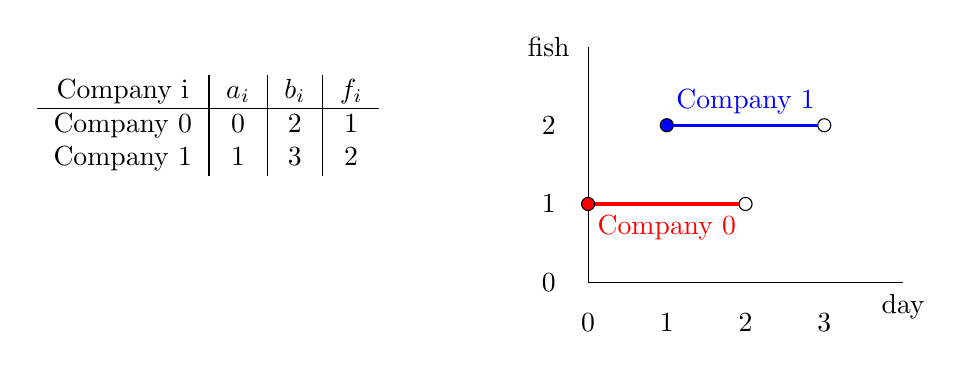
\begin{tikzpicture}
\begin{scope}[xshift=-5cm, yshift=2cm]
\node{ \begin{minipage}{4cm}
\begin{tabular}{c|c|c|c}
Company i & $a_i$ & $b_i$ & $f_i$ \\ \hline
Company 0 & 0 & 2 & 1 \\
Company 1 & 1 & 3 & 2
\end{tabular}
\end{minipage}};
\end{scope}
\draw (0,0) -- (4,0);
\draw (0,0) -- (0,3);
\foreach \i in {0,1,2,3}
{
	\node at (\i,-.5) {\i};
}
\foreach \i in {0,1,2}
{
	\node at (-.5, \i) {\i};
}
\node[draw,fill=red, circle, scale=0.5](a0) at (0,1) {};
\node[draw,fill=white, circle, scale=0.5](b0) at (2,1) {};
\draw[red, very thick] (a0) -- (b0);
\node[draw,fill=blue, circle, scale=0.5](a1) at (1,2) {};
\node[draw,fill=white, circle, scale=0.5](b1) at (3,2) {};
\draw[blue, very thick] (a1) -- (b1);
\node[red] at (1,0.7) {Company 0};
\node[blue] at (2, 2.3) {Company 1};
\node at (4,-.3) {day};
\node at (-.5, 3) {fish};
\end{tikzpicture}
\end{center}

In this example, Plucky would work for Company 0 at day $0$, and receive one fish.  He'd work for Company 1 on days $1,2$, and receive two fish on each of those days.  On days $3$ and onwards, no company was interested in Plucky's work, so he works for no company and receives zero fish.
So his output plot would look like this:
\begin{center}
\begin{tikzpicture}
\node at (4,-.3) {day};
\node at (-.5, 3) {fish};
\draw (0,0) -- (4,0);
\draw (0,0) -- (0,3);
\foreach \i in {0,1,2,3}
{
	\node at (\i,-.5) {\i};
}
\foreach \i in {0,1,2}
{
	\node at (-.5, \i) {\i};
}
\node[draw,fill=black, circle, scale=0.5](a0) at (0,1) {};
\node[draw,fill=white, circle, scale=0.5](b0) at (1,1) {};
\draw[black, very thick] (a0) -- (b0);
\node[draw,fill=black, circle, scale=0.5](a1) at (1,2) {};
\node[draw,fill=white, circle, scale=0.5](b1) at (3,2) {};
\node[draw,fill=black, circle, scale=0.5](b) at (3,0) {};
\draw[black,very thick] (b) -- (4,0);
\draw[black, very thick] (a1) -- (b1);
\end{tikzpicture}
\end{center}

To return this plot, Plucky will return a sequence $(t_0, f_0), (t_1, f_1), \ldots$, with $t_i \leq t_{i+1}$, which we interpret as meaning ``starting on day $t_i$ and ending on day $t_{i+1} - 1$, Plucky makes $f_i$ fish.  In the example above, the return value would be $(t_0 =0, f_0 = 1), (t_1 = 1, f_1 = 2), (t_2 = 3, f_2 = 0)$.  

\vspace{.5cm}
\textbf{Notes:} 
\begin{itemize}
\item The last $f$-value will always be $0$.
\item In the example above, it would also be correct to return $(t_0 = 0, f_0 = 4), (t_1 = 0, f_1 = 1), (t_2 = 1, f_2 = 2), (t_3 = 3, f_3 = 0)$; that is, adding extraneous intervals of length $0$ is still correct.
\item In the example above, it would also be correct to return $(t_0 = 0, f_0 = 1), (t_1 = 1, f_1 = 2), (t_2 =2, f_2 = 2), (t_3 = 3, f_3 = 0)$; that is, breaking an interval into two smaller intervals is still correct.
\end{itemize}
}}


\vspace{1cm}
In this problem you'll design an algorithm for Plucky.   Your algorithm should take as input a list of $n$ bids $(a_i, b_i, f_i)$, one for each company $i \in \{0,\ldots,n-1\}$, and return a list \texttt{fishPlot} of $(t_i, f_i)$ pairs as described in the example above. 

\begin{enumerate}
	\item\pts{2} Describe a simple $O(n^2)$-time algorithm for Plucky.  

	\expecting{Pseudocode, and a short English description explaining the main idea of the algorithm.  No justification of the correctness or running time is required.}

	\item\pts{6} Design a divide-and-conquer algorithm that takes time $O(n \log(n) )$. 

	\expecting{Pseudocode, and a short English description explaining the main idea of the algorithm.  We are also expecting an informal justification of correctness and of the running time.}
\end{enumerate}

\end{enumerate}
\end{document}
